Sumber data terbagi menjadi dua yaitu data primer dan data sekunder. Data primer adalah data yang diperoleh peneliti secara langsung (dari tangan pertama), sementara data sekunder adalah data yang diperoleh peneliti dari sumber yang sudah ada. Sumber data penelitian yaitu sumber subjek dari tempat mana data bisa didapatkan. Adapun data yang digunakan dalam penelitian ini adalah kuantitatif, Data kuantitatif adalah data yang dapat diinput ke dalam skala pengukuran statistik. Fakta dan fenomena dalam data ini tidak dinyatakan dalam bahasa alami, melainkan dalam numerik.





\section{Jenis Dan Sumber Data}
Pada obyek study penilitian ini menggunakan data-data yang dihasilkan dari observasi langsung dan sebagian data yang di ambil dari google maps. Data yang diperoleh yaitu data nilai dari latitude, data nila longitude, jarak, perkiraan (menit), dan titik lokasi. Tentunya dengan bantuan google maps untuk keterangan selanjutnya. Data tersebut digunakan untuk menghitung dan mencari nilai maksimum untuk mendapatkan rute terdekat menuju daerah wisata yang di tuju oleh wisatawan baik dari lokal maupun mancanegara. Rute yang di hasilkan dari sistem merupakan hasil proses perbandingan dan pengujian menggunakan komparasi Algoritma Dijkstra dan Floyd Warshall. Data wisata dikumpulkan dan di inputkan kedalam sistem, kemudian sistem dengan algoritma masing-masing akan melakukan eksekusi dan menampilkan hasil yang akurat dari proses masing-masing algoritma.

Pada penelitian ini data yang digunakan sebagai sample untuk analisis adalah rute yang dibuat di area Politeknik Pos Indonesia. Untuk analisis, data sample digunakan untuk mengetahui fungsi dan rumus dari alur algoritma tersebut. Selanjutnya untuk peng-implementasian kedua algoritma diuji dalam bentuk sistem informasi berbasis web. Kemudian data tersebut dikumpulkan dan dikelompokkan menjadi data primer dan data skunder.

\subsection{Data Primer}
\par Penelitian ini menggunakan data primer yang digunakan untuk mencari rute terdekat dalam pengolahan data menggunakan algoritma Floyd-Warshall. Pengumpulan data bertujuan untuk pengambilan data yang akan dianalisis yang kemudian dikumpulkan dan dipetakan dalam bentuk table agar mudah untuk dikelola, data diperoleh dari survey ke tempat langsung dan beberapa data lainnya di ambil dari google maps. Dari data tersebut dikumpulkan dan kemudian akan diproses pada tahap selanjutnya dalam pemodelan graf (Matriks Berbobot). Adapun data yang diperoleh dapat dilihat pada table \ref{table21}.
\par Untuk table \ref{table21} merupakan data lokasi tentang titik-titik lokasi dan jarak serta perkiraan dari jarak satu ke jarak lainnya. Untuk lokasi awal itu merupakan titik pertama kemudian lokasi akhir merupakan titik tujuan dimana titik awal dan akhir saling berkesinambungan sehingga akan membentuk sebuah graf. Untuk jarak diperoleh dari google maps sedangkan perkirann waktu sampai, dari titik awal dan akhir di peroleh dari timer penulis yang menuju dari titik awal ke titik akhir.
    
    \begin{table}[!htbp]
        \centering
        \caption{Data Jarak dan Perkiraan Lokasi}
        \label{table21}
        \begin{tabular}{|l|l|l|}
        \hline
            Node Jarak & Node Akhir & Jarak (m) \\
        \hline
            0 & 1 & 543 \\
        \hline
            0 & 5 & 742 \\
        \hline
            1 & 2 & 1827 \\
        \hline
            1 & 4 & 945 \\
        \hline
            2 & 3 & 1119 \\
        \hline
            3 & 7 & 647 \\
        \hline
            4 & 3 & 1152 \\
        \hline
            5 & 6 & 778 \\
        \hline
            6 & 7 & 1416 \\
        \hline
        \end{tabular}
    \end{table}
    
    
    
    
    
\subsection{Data Sekunder}
\par Data sekunder didapatkan dari Google Map. Data yang didapatkan dari Google Map yaitu rute-rute yang menghubungkan antara titik awal dengan titik yang akan dituju, serta jarak antar titik tiap jalannya. Data sekunder yang di miliki pada penelitian ini yaitu longitude latitude, graf lokasi, dan jalur lokasi. Data longtitude dan latitude di peroleh dengan cara mengakses google maps dan mengklik titik-titik lokasi yang akan dilalui. Untuk data lokasi longtitude dan latitude dapat dilihat pada table \ref{table22}:
    
\begin{table}[!htbp]
    \centering
    \caption{Data Longtitude dan Latitude}
    \label{table22}
    \begin{tabular}{|l|l|}
    \hline
        Titik Lokasi & Longtitude, Latitude \\
    \hline
        0 & -6.932966230283786, 107.62561082839966 \\
    \hline
        1 & -6.936885556542032, 107.62269258499146 \\
    \hline
        2 & -6.937524574035396, 107.60617017745972 \\
    \hline
        3 & -6.927470598347902, 107.60634183883667 \\
    \hline
        4 & -6.9319437919845655, 107.61574029922485 \\
    \hline
        5 & -6.929600695849448, 107.61981725692749 \\
    \hline
        6 & -6.922613940071385, 107.6199460029602 \\
    \hline
        7 & -6.921761889605031, 107.6071572303772 \\
    \hline
    \end{tabular}
\end{table}
    
\par Pada  tahap  pemodelan  graf,  data  yang  ada  diberikan  beberapa  perlakuan sehingga  membentuk  sebuah  graf  yang  dibutuhkan  oleh  penelitian  ini. Dari titik lokasi yang dikumpulkan, kemudian dihubungkan sesuai dengan titik awal dan akhir pada table \ref{table21} yang kemudian membentuk sebuah graf berbobot. Graf yang akan dihasilkan diperoleh dari proses pada table 1.1 dan table 1.2, serta jalur yang terbentuk dapat dilihat pada gambar \ref{gambar22}.
    
\begin{figure}[h]
    \centering
    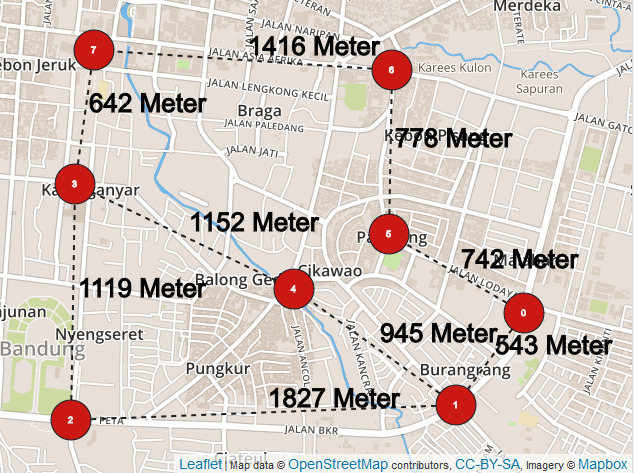
\includegraphics[scale=0.3]{figures/ALGORITMA/DATAMAP2.jpeg}
    \caption{Jalur Lokasi}
    \label{gambar22}
\end{figure}
    
\par Untuk jalur gambar \ref{gambar22} sudah terdapat bobot nilai yang tercantum yaitu jarak antara titik satu ke titik lainnya, bobot nilai ini akan di kumpulkan dan dibentuk kedalam table matriks agar dapat di proses pada tahap selanjutnya.
    
    
    
    

\section{Pemodelan Graf (Matriks Berbobot)}
\label{pemodelan_graf}
Pemodelan graf adalah graf yang setiap sisinya diberi sebuah bobot. Bobot pada tiap sisi dapat berbeda-beda bergantung pada masalah yang dimodelkan dengan graf. Bobot dapat menyatakan jarak antara dua buah kota atau titik, biaya perjalanan antara dua buah kota, waktu tempuh dari sebuah simpul ke simpul lain, ongkos produksi, dan sebagainya. Pemodelan graf dibentuk atas dasar sample data yang telah di kumpukan, dimana titik awal dan titik tujuan di hubungkan dengan bobot nilai tertentu kemudian membentuk sebuah jalur dalam bentuk graf. Secara umum sebelum dilakukan iterasi, algoritma sudah mengidenfikasi jarak terdekat dari node terdekatnya. Jika seluruh node berbobot tertentu yang (positif), maka node terdekat berikutnya dari node asal dapat ditemukan selama node berdekatan dengan node awal. Untuk graf yang dihasilkan dapat dilihat pada gambar \ref{gambar13}:

\begin{figure}[h]
    \centering
    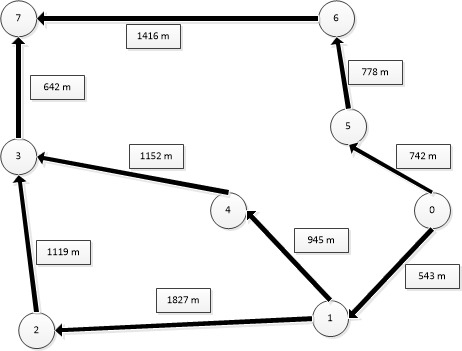
\includegraphics[scale=0.4]{figures/ALGORITMA/GRAF2.png}
    \caption{Graf Berbobot}
    \label{gambar13}
\end{figure}

\par Graf di atas dapat dilihat bahwa x adalah titik awal dan y adalah titik akhir. Graf di atas merupakan graf satu arah, hubungan graf diperoleh dari gambar \ref{gambar13}, dengan nilai jarak dan hubungan dari titik awal menuju titik akhir atau titik lainnya. Untuk matriks yang dihasilkan dari graf gambar \ref{gambar13}, dapat dilihat pada table matriks \ref{table13}:
\par Pada matriks dibawah merupakan gambaran dari graf berbobot dalam bentuk table matriks hubungan graf. Terdapat nilai yang diperoleh dari graf dan data dari hasil pengumpulan data lokasi dari google maps dan jarak yang diperoleh lalu dituliskan sesuai dengan data dari google maps dengan menghubungkan sumbu x sebagai awal dan sumbu y sebagai tujuan akhir jalur. Table matriks ini bernilai dengan satuan meter (m) dan untuk simbol "-" merupakan jarak yang tidak terjangkau atau tidak ada jalur terhadap titik tersebut.

\vspace{1cm}

\begin{table}[!htbp]
    \centering
    \caption{Matriks Hubungan Graf}
    \label{table13}
    \begin{tabular}{|l|l|l|l|l|l|l|l|l|}
    \hline
        & 0 & 1 & 2 & 3 & 4 & 5 & 6 & 7 \\
    \hline
        0 & 0 & 543 & - & - & - & 742 & - & - \\
    \hline
        1 & - & 0 & 1827 & - & 945 & - & - & - \\
    \hline
        2 & - & - & 0 & 1119 & - & - & - & - \\
    \hline
        3 & - & - & - & 0 & - & - & - & 647 \\
    \hline
        4 & - & - & - & 1152 & 0 & - & - & - \\
    \hline
        5 & - & - & - & - & - & 0 & 778 & - \\
    \hline
        6 & - & - & - & - & - & - & 0 & 1416 \\
    \hline
        7 & - & - & - & - & - & - & - & 0 \\
    \hline
    \end{tabular}
\end{table}
